% Options for packages loaded elsewhere
\PassOptionsToPackage{unicode}{hyperref}
\PassOptionsToPackage{hyphens}{url}
%
\documentclass[
]{book}
\usepackage{amsmath,amssymb}
\usepackage{iftex}
\ifPDFTeX
  \usepackage[T1]{fontenc}
  \usepackage[utf8]{inputenc}
  \usepackage{textcomp} % provide euro and other symbols
\else % if luatex or xetex
  \usepackage{unicode-math} % this also loads fontspec
  \defaultfontfeatures{Scale=MatchLowercase}
  \defaultfontfeatures[\rmfamily]{Ligatures=TeX,Scale=1}
\fi
\usepackage{lmodern}
\ifPDFTeX\else
  % xetex/luatex font selection
\fi
% Use upquote if available, for straight quotes in verbatim environments
\IfFileExists{upquote.sty}{\usepackage{upquote}}{}
\IfFileExists{microtype.sty}{% use microtype if available
  \usepackage[]{microtype}
  \UseMicrotypeSet[protrusion]{basicmath} % disable protrusion for tt fonts
}{}
\makeatletter
\@ifundefined{KOMAClassName}{% if non-KOMA class
  \IfFileExists{parskip.sty}{%
    \usepackage{parskip}
  }{% else
    \setlength{\parindent}{0pt}
    \setlength{\parskip}{6pt plus 2pt minus 1pt}}
}{% if KOMA class
  \KOMAoptions{parskip=half}}
\makeatother
\usepackage{xcolor}
\usepackage{color}
\usepackage{fancyvrb}
\newcommand{\VerbBar}{|}
\newcommand{\VERB}{\Verb[commandchars=\\\{\}]}
\DefineVerbatimEnvironment{Highlighting}{Verbatim}{commandchars=\\\{\}}
% Add ',fontsize=\small' for more characters per line
\usepackage{framed}
\definecolor{shadecolor}{RGB}{248,248,248}
\newenvironment{Shaded}{\begin{snugshade}}{\end{snugshade}}
\newcommand{\AlertTok}[1]{\textcolor[rgb]{0.94,0.16,0.16}{#1}}
\newcommand{\AnnotationTok}[1]{\textcolor[rgb]{0.56,0.35,0.01}{\textbf{\textit{#1}}}}
\newcommand{\AttributeTok}[1]{\textcolor[rgb]{0.13,0.29,0.53}{#1}}
\newcommand{\BaseNTok}[1]{\textcolor[rgb]{0.00,0.00,0.81}{#1}}
\newcommand{\BuiltInTok}[1]{#1}
\newcommand{\CharTok}[1]{\textcolor[rgb]{0.31,0.60,0.02}{#1}}
\newcommand{\CommentTok}[1]{\textcolor[rgb]{0.56,0.35,0.01}{\textit{#1}}}
\newcommand{\CommentVarTok}[1]{\textcolor[rgb]{0.56,0.35,0.01}{\textbf{\textit{#1}}}}
\newcommand{\ConstantTok}[1]{\textcolor[rgb]{0.56,0.35,0.01}{#1}}
\newcommand{\ControlFlowTok}[1]{\textcolor[rgb]{0.13,0.29,0.53}{\textbf{#1}}}
\newcommand{\DataTypeTok}[1]{\textcolor[rgb]{0.13,0.29,0.53}{#1}}
\newcommand{\DecValTok}[1]{\textcolor[rgb]{0.00,0.00,0.81}{#1}}
\newcommand{\DocumentationTok}[1]{\textcolor[rgb]{0.56,0.35,0.01}{\textbf{\textit{#1}}}}
\newcommand{\ErrorTok}[1]{\textcolor[rgb]{0.64,0.00,0.00}{\textbf{#1}}}
\newcommand{\ExtensionTok}[1]{#1}
\newcommand{\FloatTok}[1]{\textcolor[rgb]{0.00,0.00,0.81}{#1}}
\newcommand{\FunctionTok}[1]{\textcolor[rgb]{0.13,0.29,0.53}{\textbf{#1}}}
\newcommand{\ImportTok}[1]{#1}
\newcommand{\InformationTok}[1]{\textcolor[rgb]{0.56,0.35,0.01}{\textbf{\textit{#1}}}}
\newcommand{\KeywordTok}[1]{\textcolor[rgb]{0.13,0.29,0.53}{\textbf{#1}}}
\newcommand{\NormalTok}[1]{#1}
\newcommand{\OperatorTok}[1]{\textcolor[rgb]{0.81,0.36,0.00}{\textbf{#1}}}
\newcommand{\OtherTok}[1]{\textcolor[rgb]{0.56,0.35,0.01}{#1}}
\newcommand{\PreprocessorTok}[1]{\textcolor[rgb]{0.56,0.35,0.01}{\textit{#1}}}
\newcommand{\RegionMarkerTok}[1]{#1}
\newcommand{\SpecialCharTok}[1]{\textcolor[rgb]{0.81,0.36,0.00}{\textbf{#1}}}
\newcommand{\SpecialStringTok}[1]{\textcolor[rgb]{0.31,0.60,0.02}{#1}}
\newcommand{\StringTok}[1]{\textcolor[rgb]{0.31,0.60,0.02}{#1}}
\newcommand{\VariableTok}[1]{\textcolor[rgb]{0.00,0.00,0.00}{#1}}
\newcommand{\VerbatimStringTok}[1]{\textcolor[rgb]{0.31,0.60,0.02}{#1}}
\newcommand{\WarningTok}[1]{\textcolor[rgb]{0.56,0.35,0.01}{\textbf{\textit{#1}}}}
\usepackage{longtable,booktabs,array}
\usepackage{calc} % for calculating minipage widths
% Correct order of tables after \paragraph or \subparagraph
\usepackage{etoolbox}
\makeatletter
\patchcmd\longtable{\par}{\if@noskipsec\mbox{}\fi\par}{}{}
\makeatother
% Allow footnotes in longtable head/foot
\IfFileExists{footnotehyper.sty}{\usepackage{footnotehyper}}{\usepackage{footnote}}
\makesavenoteenv{longtable}
\usepackage{graphicx}
\makeatletter
\def\maxwidth{\ifdim\Gin@nat@width>\linewidth\linewidth\else\Gin@nat@width\fi}
\def\maxheight{\ifdim\Gin@nat@height>\textheight\textheight\else\Gin@nat@height\fi}
\makeatother
% Scale images if necessary, so that they will not overflow the page
% margins by default, and it is still possible to overwrite the defaults
% using explicit options in \includegraphics[width, height, ...]{}
\setkeys{Gin}{width=\maxwidth,height=\maxheight,keepaspectratio}
% Set default figure placement to htbp
\makeatletter
\def\fps@figure{htbp}
\makeatother
\setlength{\emergencystretch}{3em} % prevent overfull lines
\providecommand{\tightlist}{%
  \setlength{\itemsep}{0pt}\setlength{\parskip}{0pt}}
\setcounter{secnumdepth}{5}
\usepackage{booktabs}
\ifLuaTeX
  \usepackage{selnolig}  % disable illegal ligatures
\fi
\usepackage[]{natbib}
\bibliographystyle{apalike}
\IfFileExists{bookmark.sty}{\usepackage{bookmark}}{\usepackage{hyperref}}
\IfFileExists{xurl.sty}{\usepackage{xurl}}{} % add URL line breaks if available
\urlstyle{same}
\hypersetup{
  pdftitle={Lerne Python, indem du Spiele entwickels},
  pdfauthor={Alexander (Sasha) Pastukhov},
  hidelinks,
  pdfcreator={LaTeX via pandoc}}

\title{Lerne Python, indem du Spiele entwickels}
\author{Alexander (Sasha) Pastukhov}
\date{2023-10-06}

\begin{document}
\maketitle

{
\setcounter{tocdepth}{1}
\tableofcontents
}
\hypertarget{intro}{%
\chapter{Einleitung}\label{intro}}

Dieses Buch wird dich das Programmieren lehren. Hoffentlich auf eine spaßige Art und Weise, denn wenn es etwas Befriedigenderes gibt als ein Videospiel zu spielen, dann ist es, eines zu erstellen. Obwohl es für den Kurs \emph{``Python für soziale und experimentelle Psychologie''} geschrieben wurde, ist mein Hauptziel nicht, dir Python an sich beizubringen. Python ist ein fantastisches Werkzeug (mehr dazu später), aber es ist nur eine von vielen existierenden Programmiersprachen. Mein ultimatives Ziel ist es, dir dabei zu helfen, allgemeine Programmierfähigkeiten zu entwickeln, die nicht von einer spezifischen Programmiersprache abhängen, und sicherzustellen, dass du gute Gewohnheiten entwickelst, die deinen Code klar, leicht lesbar und leicht zu warten machen. Dieser letzte Teil ist entscheidend. Programmieren geht nicht nur darum, Code zu schreiben, der funktioniert. Das muss natürlich gegeben sein, ist aber nur die Mindestanforderung. Programmieren geht darum, einen klaren und leicht lesbaren Code zu schreiben, den andere und, noch wichtiger, du selbst zwei Wochen später verstehen kannst.

\hypertarget{ziel-des-buches}{%
\section{Ziel des Buches}\label{ziel-des-buches}}

Das Ziel ist, dass du in der Lage bist, ein anspruchsvolles Experiment zu programmieren, das mehrere Blöcke und Versuche, verschiedene Bedingungen, komplizierte visuelle Darstellungen, automatische Datenaufzeichnung und Fehlerbehandlung haben kann. Wenn das ambitioniert klingt, dann ist es das auch, aber wir werden in kleinen Schritten vorgehen und im Prozess wirst du lernen.

\begin{itemize}
\tightlist
\item
  Kernkonzepte von Python einschließlich

  \begin{itemize}
  \tightlist
  \item
    Variablen und Konstanten
  \item
    unveränderliche Datentypen wie Ganzzahlen, Fließkommazahlen, Zeichenketten, logische Werte und Tupel
  \item
    veränderliche Typen wie Listen und Dictionaries
  \item
    Funktionen
  \item
    Steuerungsstrukturen wie if-else-Bedingungen und Schleifen
  \item
    objektorientierte Programmierung einschließlich Konzepte des Vererbung, (optional) Duck-Typing und Mischung
  \item
    Ausnahmen
  \item
    Dateioperationen
  \end{itemize}
\item
  PsychoPy: Dies ist nicht Kern-Python, aber es ist eine erstklassige Bibliothek für psychophysische Experimente und du wirst die Schlüsselwerkzeuge lernen, die für die Programmierung eines Experiments erforderlich sind.
\item
  Guter Programmierstil einschließlich

  \begin{itemize}
  \tightlist
  \item
    Klaren Code in iterativer Weise schreiben
  \item
    Lesen (deines eigenen) Codes
  \item
    Dokumentieren deines Codes
  \item
    Debuggen deines Programms in VS Code
  \end{itemize}
\end{itemize}

Ich habe versucht, Konzepte in dem Kontext zu präsentieren, der sie erfordert und daher am besten erklärt und ihre typischen Anwendungsszenarien darstellt. Das bedeutet, dass das Material rund um verteilt ist und auf Bedarfsbasis präsentiert wird. Zum Beispiel wird das Konzept der Listen zuerst präsentiert, aber Operationen daran werden in einem späteren Kapitel vorgestellt, sowohl weil wir dies erst später benötigen als auch um dein Gefühl, überwältigt zu sein, in einem vernünftigen Rahmen zu halten. Dies macht es schwieriger, dieses Buch als Referenz zu verwenden (es gibt ausgezeichnete Referenzen da draußen, angefangen mit der \href{https://docs.python.org/3/}{offiziellen Python-Dokumentation}), aber die Hoffnung ist, dass es dir durch die Bereitstellung von mundgerechten Informationsbrocken leichter fallen wird, das Material zu verstehen und es mit dem zu integrieren, was du bereits weißt.

Die gleiche ``verteilte'' Logik gilt für Übungen. Anstatt am Ende jedes Kapitels aufgelistet zu sein, sind sie in den Text eingebettet und du solltest sie zu diesem Zeitpunkt erledigen. Viele von ihnen dienen dazu, Konzepte zu verdeutlichen, die zuvor anhand von anschaulichen Beispielen präsentiert wurden, daher wäre es hilfreich, sie sofort durchzuführen. Gleiches gilt für die Programmierübung, obwohl du in diesem Fall das gesamte Material lesen kannst, um eine ``Vogelperspektive'' auf das gesamte Programm zu bekommen und dann den Text erneut zu lesen und die Programmierübung durchzuführen.

\hypertarget{voraussetzungen}{%
\section{Voraussetzungen}\label{voraussetzungen}}

Dieses Material setzt keine Vorkenntnisse in Python oder Programmierung beim Leser voraus. Sein Ziel ist es, dein Wissen schrittweise aufzubauen und dir zu ermöglichen, immer komplexere Spiele zu erstellen.

\hypertarget{warum-spiele}{%
\section{Warum Spiele?}\label{warum-spiele}}

Der eigentliche Zweck dieses Kurses ist es, Psychologie- und Sozialwissenschaftsstudenten beizubringen, wie man \emph{Experimente} programmiert. Das ist es, worum es in der echten Forschung geht. Allerdings gibt es zwischen den beiden praktisch wenig Unterschied. Die grundlegenden Zutaten sind die gleichen und, man könnte sagen, Experimente sind einfach nur langweilige Spiele. Und sei versichert, wenn du ein Spiel programmieren kannst, kannst du sicherlich auch ein Experiment programmieren.

\hypertarget{warum-sollte-ein-psychologe-programmieren-lernen}{%
\section{Warum sollte ein Psychologe Programmieren lernen?}\label{warum-sollte-ein-psychologe-programmieren-lernen}}

Warum sollte ein Psychologe, der an Menschen interessiert ist, lernen, wie man Computer programmiert? Die offensichtlichste Antwort ist, dass dies eine nützliche Fähigkeit ist. Wenn du programmieren kannst, hast du die Freiheit, ein Experiment zu erstellen, das deine Forschungsfrage beantwortet, und nicht ein Experiment, das aufgrund der Beschränkungen deiner Software implementiert werden kann.

Noch wichtiger, zumindest aus meiner Sicht, ist, dass das Erlernen des Programmierens die Art und Weise, wie du im Allgemeinen denkst, verändert. Menschen sind klug, aber Computer sind dumm\footnote{Dies wurde geschrieben, bevor große Sprachmodelle aufkamen, aber trifft immer noch zu, wenn es ums Programmieren geht.}. Wenn du dein Experiment oder deine Reisepläne jemandem erklärst, kannst du ziemlich vage sein, einen kleinen Fehler machen, sogar bestimmte Teile überspringen. Menschen sind klug, daher werden sie die fehlenden Informationen mit ihrem Wissen ergänzen, einen Fehler finden und korrigieren, dich nach mehr Informationen fragen und selbst improvisieren können, sobald sie auf etwas stoßen, das du nicht abgedeckt hast. Computer sind dumm, also musst du präzise sein, du kannst keine Grauzonen haben, du kannst nichts dem ``es wird herausfinden, wenn es passiert'' (es wird es nicht) überlassen. Meine persönliche Erfahrung, die von Psychologen bestätigt wurde, die das Programmieren gelernt haben, ist, dass es dir bewusst macht, wie vage und ungenau Menschen sein können, ohne es zu merken (und ohne dass du es merkst). Programmieren zwingt dich dazu, präzise und gründlich zu sein, für alle Eventualitäten zu planen, die es geben könnte. Und das ist an sich eine sehr nützliche Fähigkeit, da sie auf alle Aktivitäten angewendet werden kann, die Planung erfordern, sei es ein experimentelles Design oder Reisevorkehrungen.

\hypertarget{warum-python}{%
\section{Warum Python?}\label{warum-python}}

Es gibt viele Möglichkeiten, ein Experiment für psychologische Forschung zu erstellen. Du kannst Drag-and-Drop-Systeme verwenden, entweder kommerzielle wie \href{https://www.neurobs.com/}{Presentation}, \href{https://www.sr-research.com/experiment-builder/}{Experiment Builder} oder kostenlose wie \href{https://psychopy.org/builder}{PsychoPy Builder Interface}. Sie haben eine viel flachere Lernkurve, sodass du schneller mit dem Erstellen und Durchführen deiner Experimente beginnen kannst. Ihre einfache Handhabung hat jedoch einen Preis: Sie sind recht begrenzt, welche Reize du verwenden kannst und wie du die Präsentation, Bedingungen, Feedback etc. steuern kannst. In der Regel erlauben sie dir, sie zu erweitern, indem du das gewünschte Verhalten programmierst, aber du musst wissen, wie man das macht (Python-Kenntnisse bereichern deine PsychoPy-Experimente). Daher denke ich, dass diese Systeme, insbesondere \href{https://psychopy.org/}{PsychoPy}, großartige Werkzeuge sind, um schnell ein einfaches Experiment zusammenzusetzen. Sie sind jedoch am nützlichsten, wenn du verstehst, \emph{wie} sie den zugrunde liegenden Code erstellen und wie du ihn selbst programmieren würdest. Dann wirst du nicht durch die Software eingeschränkt, da du weißt, dass du etwas programmieren kannst, was der Standard-Drag-and-Drop nicht zulässt. Gleichzeitig kannst du dich immer dafür entscheiden, wenn Drag-and-Drop ausreichend, aber schneller ist, oder du kannst eine Kombination aus beiden Ansätzen verwenden. Am Ende geht es darum, Optionen und kreative Freiheit zu haben, ein Experiment zu programmieren, das deine Forschungsfrage beantwortet, und nicht nur ein Experiment, das deine Software erlaubt zu programmieren.

Wir werden das Programmieren in Python lernen, eine großartige Sprache, die eine einfache und klare Syntax mit der Kraft und Fähigkeit kombiniert, fast jedes Problem zu bewältigen. In diesem Seminar konzentrieren wir uns auf Desktop-Experimente, aber Sie können es für Online-Experimente (\href{https://otree.readthedocs.io/en/latest/}{oTree} und \href{https://psychopy.org/}{PsychoPy}), wissenschaftliche Programmierung (\href{https://numpy.org/}{NumPy} und \href{https://www.scipy.org/}{SciPy}), Datenanalyse (\href{https://pandas.pydata.org/}{pandas}), Maschinelles Lernen (\href{https://scikit-learn.org/}{scikit-learn}), Deep Learning (\href{https://keras.io/}{keras}), Website-Programmierung (\href{https://www.djangoproject.com/}{django}), Computer Vision (\href{https://opencv.org/}{OpenCV}) usw. verwenden. Daher ist Python eines der vielseitigsten Programmierwerkzeuge, die Sie für alle Phasen Ihrer Forschung oder Arbeit verwenden können. Und Python ist kostenlos, so dass Sie sich keine Sorgen machen müssen, ob Sie oder Ihr zukünftiger Arbeitgeber die Lizenzgebühren bezahlen können (ein sehr reales Problem, wenn Sie Matlab verwenden).

\hypertarget{seminar-spezifische-informationen}{%
\section{Seminar-spezifische Informationen}\label{seminar-spezifische-informationen}}

Dies ist ein Material für das Seminar \emph{Python für Sozial- und Experimentelle Psychologie}, wie ich es an der Universität Bamberg lehre. Jedes Kapitel behandelt ein einzelnes Spiel und führt die notwendigen Ideen ein und wird von Übungen begleitet, die Sie absolvieren und einreichen müssen. Um das Seminar zu bestehen, müssen Sie alle Aufgaben absolvieren, d.h., alle Spiele schreiben. Sie müssen nicht alle Übungen abschließen oder korrekte Lösungen für \emph{alle} Übungen liefern, um den Kurs zu bestehen und Informationen darüber, wie die Punkte für Übungen in eine tatsächliche Note (falls Sie eine benötigen) oder ``Bestanden'' umgerechnet werden, werden während des Seminars verfügbar sein.

Das Material ist so strukturiert, dass jedes Kapitel oder Kapitelabschnitt typischerweise einer einzelnen Sitzung entspricht, außer für die abschließenden Kapitel, die auf komplexeren Spielen basieren und daher mehr Zeit in Anspruch nehmen. Wir sind jedoch alle verschieden, also arbeiten Sie in Ihrem eigenen Tempo, lesen Sie das Material und reichen Sie Aufgaben eigenständig ein. Ich werde für jede Aufgabe detailliertes Feedback geben und Ihnen die Möglichkeit bieten, Probleme anzugehen und erneut einzureichen, ohne Punkte zu verlieren. Beachten Sie, dass mein Feedback nicht nur die tatsächlichen Probleme mit dem Code abdeckt, sondern auch die Art und Weise, wie Sie die Lösung implementiert haben und wie sauber und gut dokumentiert Ihr Code ist. Denken Sie daran, unsere Aufgabe ist es nicht nur, zu lernen, wie man ein funktionierendes Spiel programmiert, sondern wie man einen schönen, klaren, leicht zu lesenden und zu wartenden Code schreibt\footnote{Gute Gewohnheiten! Bilden Sie gute Gewohnheiten! Danke, dass Sie diese unterschwellige Botschaft gelesen haben.}.

Sehr wichtig: Zögern Sie nicht, Fragen zu stellen. Wenn ich das Gefühl habe, dass Sie die Informationen im Material übersehen haben, werde ich Sie auf die genaue Stelle hinweisen. Wenn Sie verwirrt sind, werde ich Sie sanft mit Fragen dazu anregen, Ihr eigenes Problem zu lösen. Wenn Sie mehr Informationen benötigen, werde ich diese liefern. Wenn Sie einfach mehr wissen wollen, fragen Sie und ich werde erklären, warum die Dinge so sind, wie sie sind, oder vorschlagen, was Sie lesen sollten. Wenn ich das Gefühl habe, dass Sie das Problem ohne meine Hilfe lösen können, werde ich Ihnen das sagen (obwohl ich wahrscheinlich trotzdem noch ein paar andeutende Fragen stellen würde).

\hypertarget{uxfcber-das-material}{%
\section{Über das Material}\label{uxfcber-das-material}}

Dieses Material ist \textbf{kostenlos zu nutzen} und steht unter der Lizenz \href{https://creativecommons.org/licenses/by-nc-nd/4.0/}{Creative Commons Namensnennung-NichtKommerziell-KeineBearbeitung V4.0 International Lizenz}.

\hypertarget{Software}{%
\chapter{Software}\label{Software}}

Für dieses Buch und das Seminar müssen wir installieren

\begin{itemize}
\tightlist
\item
  PsychoPy.
\item
  IDE Ihrer Wahl. Meine Anleitungen werden für Visual Studio Code sein, das eine sehr gute Python-Unterstützung bietet.
\item
  Jupyter Notebook zum Ausprobieren kleiner Code-Snippets.
\end{itemize}

Ich werde keine detaillierten Anleitungen zur Installation der notwendigen Software geben, sondern Sie eher auf die offiziellen Handbücher verweisen. Dies macht diesen Text zukunftssicherer, da sich spezifische Details leicht ändern könnten\footnote{Wenn Sie Teil des Seminars sind, fragen Sie mich, wann immer Sie Probleme haben oder unsicher sind, wie Sie vorgehen sollen}.

\hypertarget{install-psychopy}{%
\section{PsychoPy}\label{install-psychopy}}

Wenn Sie Windows verwenden, laden Sie die \href{https://www.psychopy.org/download.html}{Standalone PsychoPy} Version herunter und installieren Sie diese. Verwenden Sie die neueste (und beste) Ihnen vorgeschlagene PsychoPy-Version (PsychoPy 2023.2.2 mit Python 3.8 zum Zeitpunkt des Schreibens) und folgen Sie den Anweisungen.

Wenn Sie Mac oder Linux verwenden, sind die Installation von PsychoPy über pip oder Anaconda Ihre Optionen. Bitte folgen Sie den aktuellen \href{https://www.psychopy.org/download.html\#manual-installations}{Anweisungen}.

\hypertarget{install-vs-code}{%
\section{VS Code}\label{install-vs-code}}

\href{https://code.visualstudio.com/}{Visual Studio Code} ist ein kostenloser, leichtgewichtiger Open-Source-Editor mit starker Unterstützung für Python. Laden Sie den Installer für Ihre Plattform herunter und folgen Sie den Anweisungen.

Befolgen Sie als nächstes das Tutorial \href{https://code.visualstudio.com/docs/python/python-tutorial}{Getting Started with Python in VS Code}. Wenn Sie Windows und die Standalone-Installation von PsychoPy verwenden, \textbf{überspringen} Sie den Abschnitt \emph{Install a Python interpreter}, da Sie bereits eine Python-Installation haben, die mit PsychoPy gebündelt ist. Dies ist der Interpreter, den Sie im Abschnitt \emph{Select a Python interpreter} verwenden sollten. In meinem Fall ist der Pfad \texttt{C:\textbackslash{}Program\ Files\textbackslash{}PsychoPy3\textbackslash{}python.exe}.

Installieren und aktivieren Sie einen Linter, eine Software, die syntaxtische und stilistische Probleme in Ihrem Python-Quellcode hervorhebt. Folgen Sie dem \href{https://code.visualstudio.com/docs/python/linting}{Handbuch} auf der Webseite von VS Code.

\hypertarget{jupyter-notebooks}{%
\section{Jupyter Notebooks}\label{jupyter-notebooks}}

\href{https://jupyter.org/}{Jupyter Notebooks} bieten eine sehr bequeme Möglichkeit, Text, Bilder und Code in einem einzigen Dokument zu mischen. Sie erleichtern auch das Ausprobieren verschiedener kleiner Code-Snippets parallel ohne das Ausführen von Skripten. Wir werden uns für unser erstes Kapitel und gelegentliche Übungen oder Code-Tests später darauf verlassen. Es gibt zwei Möglichkeiten, wie Sie sie verwenden können: 1) in VS Code mit der Jupyter-Erweiterung, 2) in Ihrem Browser mit der klassischen Oberfläche.

\hypertarget{jupyter-notebooks-in-vs-code}{%
\subsection{Jupyter Notebooks in VS Code}\label{jupyter-notebooks-in-vs-code}}

Folgen Sie \href{https://code.visualstudio.com/docs/datascience/jupyter-notebooks}{der Anleitung}, wie Sie das Jupyter-Paket installieren und Notebooks in VS Code verwenden.

\hypertarget{jupyter-notebooks-in-anaconda}{%
\subsection{Jupyter Notebooks in Anaconda}\label{jupyter-notebooks-in-anaconda}}

Die einfachste Möglichkeit, Jupyter Notebooks zusammen mit vielen anderen nützlichen Data-Science-Tools zu verwenden, ist über das \href{https://www.anaconda.com/products/individual}{Anaconda} Toolkit. Beachten Sie jedoch, dass dies eine \emph{zweite} Python-Distribution in Ihrem System installiert. Dies könnte wiederum zu Verwirrung führen, wenn Sie mit Skripten in VS Code arbeiten und versehentlich den Anaconda-Interpreter statt den PsychoPy-Interpreter aktiv haben. Keine Panik, folgen Sie den \href{https://code.visualstudio.com/docs/python/python-tutorial\#_select-a-python-interpreter}{Select a Python interpreter} Anweisungen und stellen Sie sicher, dass Sie den PsychoPy-Interpreter als den aktiven haben.

Ansonsten laden Sie Anaconda herunter und installieren Sie es. Die Website hat einen ausgezeichneten \href{https://docs.anaconda.com/anaconda/user-guide/getting-started/}{Getting started} Abschnitt.

\hypertarget{files-folder}{%
\section{Ordnung halten}\label{files-folder}}

Bevor wir anfangen, schlage ich vor, dass Sie einen Ordner namens \emph{games-with-python} (oder so ähnlich) erstellen. Wenn Sie sich dafür entschieden haben, Jupyter Notebooks über Anaconda zu nutzen, sollten Sie diesen Ordner in Ihrem Benutzerordner erstellen, da Anaconda dort die Dateien erwartet. Dann erstellen Sie einen neuen Unterordner für jedes Kapitel / Spiel. Für das Seminar müssten Sie einen Ordner mit allen Dateien zippen und hochladen.

\hypertarget{programming-tips}{%
\chapter{Programmier-Tipps und -Tricks}\label{programming-tips}}

Bevor Sie Ihren ersten Code schreiben, müssen wir über die Kunst des Programmierens sprechen. Wie ich bereits erwähnt habe, geht es nicht nur darum, dass der Code funktioniert, sondern darum, dass er leicht zu verstehen ist. Korrekt funktionierender Code ist ein schönes Plus, aber wenn ich zwischen einem Spaghetti-Code, der momentan korrekt funktioniert, und einem klar geschriebenen und dokumentierten Code, der noch repariert werden muss, wählen muss, werde ich immer Letzteren bevorzugen. Ich kann Dinge reparieren, die ich verstehe, ich kann nur hoffen, wenn ich das nicht tue.

Unten sind einige Tipps zum Schreiben und Lesen von Code. Einige mögen beim ersten Lesen kryptisch klingen (sie werden klar, sobald wir das notwendige Material behandeln). Einige werden sich für die einfachen Projekte, die wir umsetzen werden, als Overkill anfühlen. Ich schlage vor, dass Sie diesen Abschnitt beim ersten Mal ungezwungen lesen, aber oft darauf zurückkommen, sobald wir ernsthaft mit Programmieren beginnen. Leider werden diese Tricks nicht funktionieren, wenn Sie sie nicht benutzen! Daher sollten Sie sie \emph{immer} benutzen und sie sollten Ihre \emph{guten Gewohnheiten} werden, wie das Anlegen eines Sicherheitsgurtes. Der Sicherheitsgurt ist an den meisten (hoffentlich allen) Tagen nicht nützlich, aber Sie tragen ihn, weil er plötzlich und sehr dringend extrem nützlich werden könnte und Sie nie sicher sein können, wann das passieren wird. Gleiches gilt für das Programmieren. Oft werden Sie versucht sein, einen ``quick-n-dirty'' Code zu schreiben, weil es sich nur um einen ``einfachen Test'', eine temporäre Lösung, einen Prototyp, ein Pilotexperiment, usw. handelt. Aber wie man so schön sagt: ``Es gibt nichts Beständigeres als eine provisorische Lösung''. Häufiger als nicht werden Sie feststellen, dass Ihr Spielzeugcode zu einem ausgewachsenen Experiment herangewachsen ist und es ein Durcheinander ist. Oder Sie möchten zu dem Pilotexperiment zurückkehren, das Sie vor ein paar Monaten durchgeführt haben, aber Sie stellen fest, dass es einfacher ist, von vorne zu beginnen, als zu verstehen, wie dieses Monster funktioniert\footnote{Mir ist das öfter passiert, als ich zugeben möchte.}. Widerstehen Sie also der Versuchung! Bilden Sie gute Gewohnheiten und Ihr zukünftiges Ich wird sehr dankbar sein!

\hypertarget{schreibtipps}{%
\section{Den Code schreiben}\label{schreibtipps}}

\hypertarget{verwende-einen-linter}{%
\subsection{Verwende einen Linter}\label{verwende-einen-linter}}

Ein Linter ist ein Programm, das deinen Code-Stil analysiert und highlightet Probleme, die es findet: unnötige Leerzeichen, fehlende Leerzeichen, falsche Namen, übermäßig lange Zeilen, usw. Diese haben keinen Einflluss darauf, wie der Code ausgeführt wird, aber das Befolgen der Linter-Ratschläge führt zu einem konsistenten Standard, wenn auch langweiligen{[}\^{} ``Langweilig ist gut!'', siehe den Film ``The Hitman's Bodyguard.''{]} Python Code. Versuche, alle Probleme zu beheben, die der Linter aufgeworfen hat. Verwende jedoch dein besseres Urteilsvermögen, denn manchmal sind Zeilen, die länger sind als der Linter es bevorzugen würde, lesbarer als zwei kürzere. Ebenso kann ein ``schlechter'' Variablenname nach den Standards des Linters für einen Psychologen eine aussagekräftige Bezeichnung sein. Denke daran, dein Code ist für Menschen, nicht für den Linter.

\hypertarget{dokumentiere-deinen-code}{%
\subsection{Dokumentiere deinen Code}\label{dokumentiere-deinen-code}}

Jedes Mal, wenn du eine neue Datei erstellst: dokumentiere sie und aktualisiere die Dokumentation, wann immer du neue Funktionen oder Klassen hinzufügst/änderst/löschst. Jedes Mal, wenn du eine neue Funktion erstellst: dokumentiere sie. Neue Klasse: dokumentiere sie. Neue Konstante: es sei denn, es ist alleine aus dem Namen klar, dokumentiere sie. Du wirst eine \href{https://numpydoc.readthedocs.io/en/latest/format.html}{NumPy} Methode der Dokumentation in dem Buch lernen.

Ich kann nicht genug betonen, wie wichtig es ist, deinen Code zu dokumentieren. VS Code (ein Editor, den wir verwenden werden) ist intelligent genug, um NumPy Docstrings zu parsen, also wird es dir diese Hilfe anzeigen, wann immer du deine eigenen Funktionen verwendest (hilft dir, dir selbst zu helfen!). Noch wichtiger ist, dass das Schreiben von Dokumentationen dich dazu zwingt, in menschlicher Sprache zu denken und zu formulieren, was die Funktion oder Klasse macht, welchen Typ die Argumente / Attribute / Methoden haben, was der Bereich der gültigen Werte ist, was die Standards sind, was eine Funktion zurückgeben sollte usw. Mehr als oft nicht, wirst du feststellen, dass du ein wichtiges Detail übersehen hast, das aus dem Code selbst nicht ersichtlich ist.

\hypertarget{fuxfcge-etwas-luft-hinzu}{%
\subsection{Füge etwas Luft hinzu}\label{fuxfcge-etwas-luft-hinzu}}

Trenne Codeblöcke durch einige leere Zeilen. Denke an Absätze im normalen Text. Du würdest nicht wollen, dass dein Buch ein einziger Absatz-Alptraum ist? Platziere vor jedem Codeblock einen Kommentar, der erklärt, \emph{was} er macht, aber nicht \emph{wie} er es macht. Zum Beispiel wird es in unserem typischen PsychoPy-basierten Spiel einen Punkt geben, an dem wir alle Reize zeichnen und das Fenster aktualisieren. Das ist ein schöner selbstständiger Codeblock, der als \texttt{\#\ Zeichnen\ aller\ Reize} beschrieben werden kann. Der Code liefert Details darüber, was genau gezeichnet wird, was die Zeichenreihenfolge ist, usw. Aber dieser einzelne Kommentar hilft dir zu verstehen, worum es in diesem Codeblock geht und ob er für dich momentan relevant ist.
Das Gleiche gilt für \texttt{\#\ Verarbeitung\ von\ Tastendrücken} oder \texttt{\#\ Überprüfung\ der\ Spielende-Bedingungen}, usw. Aber sei vorsichtig und stelle sicher, dass der Kommentar den Code korrekt beschreibt. Wenn der Kommentar zum Beispiel \texttt{\#\ Zeichnen\ aller\ Reize} sagt, sollte es nirgendwo anders einen Code zum Zeichnen von Reizen geben und keinen weiteren Code, der etwas anderes tut!

\hypertarget{schreibe-deinen-code-schritt-fuxfcr-schritt}{%
\subsection{Schreibe deinen Code Schritt für Schritt}\label{schreibe-deinen-code-schritt-fuxfcr-schritt}}

Dein Motto sollte ``langsam aber stetig'' lauten. Auf diese Weise werde ich dich durch die Spiele führen. Beginne immer mit etwas extrem Einfachem wie einem statischen Rechteck oder Bild. Stelle sicher, dass es funktioniert. Füge eine kleinere Funktionalität hinzu: Farbwechsel, Positionsänderung, ein weiteres Rechteck, speichere es als Attribut, usw. Stelle sicher, dass es funktioniert. Gehe niemals zum nächsten Schritt, es sei denn, du verstehst vollständig, was dein aktueller Code macht und du bist dir zu 100\% sicher, dass er sich so verhält, wie er sollte. Und ich meine 100\% ernst! Wenn du auch nur den Schatten eines Zweifels hast, überprüfe es erneut. Andernfalls wird dieser Schatten wachsen und dich zunehmend unsicher über deinen Code machen. Dieser Ansatz in Schildkrötengeschwindigkeit mag albern und übermäßig langsam erscheinen, ist aber immer noch schneller, als einen großen Codeblock zu schreiben und dann zu versuchen, ihn zum Laufen zu bringen. Es ist viel einfacher, einfache Probleme einzeln zu lösen, als viele auf einmal.

\hypertarget{es-ist-nichts-falsches-an-stackoverflow}{%
\subsection{Es ist nichts Falsches an StackOverflow}\label{es-ist-nichts-falsches-an-stackoverflow}}

Ja, man kann immer versuchen, eine Lösung für sein Problem auf StackOverflow zu finden\footnote{Wenn Sie jedoch an dem Seminar teilnehmen, fragen Sie mich bitte zuerst!}. Ich mache das die ganze Zeit! Sie sollten die bereitgestellte Lösung jedoch \emph{nur verwenden, wenn Sie sie verstehen}! Kopieren Sie nicht einfach den Code, der ein Problem wie Ihres zu lösen \emph{scheint}. Wenn Sie das tun und Sie haben Glück, könnte es funktionieren. Oder, wieder wenn Sie Glück haben, funktioniert es auf eine offensichtliche Weise nicht. Aber wenn Sie nicht so viel Glück haben, wird es (manchmal) subtil falsch funktionieren. Und da Sie nicht wirklich wussten, was der Code tat, als Sie ihn einfügten, werden Sie noch mehr verwirrt sein. Nutzen Sie also StackOverflow als eine Quelle des Wissens, nicht als eine Quelle zum Kopieren und Einfügen von Code!

\hypertarget{reading-tips}{%
\section{Den Code lesen}\label{reading-tips}}

Das Lesen von Code ist einfach, weil Computer dumm sind und Sie schlau sind. Das bedeutet, dass die Anweisungen, die Sie dem Computer geben, notwendigerweise sehr einfach sind und daher für einen Menschen sehr leicht zu verstehen sind. Das Lesen von Code ist jedoch auch schwierig, weil Computer dumm sind und Sie schlau sind. Sie sind so schlau, dass Sie nicht einmal den gesamten Code lesen müssen, um zu verstehen, was er tut. Sie lesen nur die Schlüsselstellen und füllen die Lücken aus. Leider neigen Sie dazu, Fehler zu überlesen. Dies ist nicht nur beim Programmieren der Fall, wenn Sie jemals einen Text Korrektur gelesen haben, wissen Sie, wie schwierig es ist, Tippfehler zu finden. Ihr Gehirn korrigiert sie in Echtzeit mit Hilfe des Kontexts und Sie lesen das Wort so, wie es sein sollte, nicht so, wie es tatsächlich geschrieben ist\footnote{Tipp: Lesen Sie Ihren Text ein Satz nach dem anderen von hinten nach vorne oder lesen Sie zufällig einen Satz nach dem anderen. Dies bricht den Fluss des Textes und hilft Ihnen, sich auf die Wörter zu konzentrieren, anstatt auf die Bedeutung und die Geschichte.}.

Meine Erfahrung mit Programmierung im Allgemeinen und im Besonderen auf diesem Seminar ist, dass die meisten Probleme, bei denen Sie stecken bleiben, im Nachhinein einfach bis dumm und offensichtlich sind\footnote{Im Nachhinein ist man immer schlauer!}. Verzweifeln Sie nicht! Es liegt nicht an Ihnen, sondern ist lediglich eine Folge davon, wie wunderbar Ihr Gehirn für die Mustererkennung verdrahtet ist. Im Folgenden finden Sie einige Vorschläge, die Ihnen helfen könnten, das Lesen von Code robuster zu gestalten.

\hypertarget{denken-sie-wie-ein-computer}{%
\subsection{Denken Sie wie ein Computer}\label{denken-sie-wie-ein-computer}}

Lesen Sie den Code Zeile für Zeile und ``führen Sie ihn aus'', so wie es der Computer tun würde. Verwenden Sie Stift und Papier, um den Überblick über die Variablen zu behalten. Verfolgen Sie, welche Codeblöcke wann erreicht werden können. Verlangsamen Sie sich und stellen Sie sicher, dass Sie jede Zeile verstehen und in der Lage sind, den Überblick über die Variablen zu behalten. Sobald Sie das tun, wird es einfach sein, einen Fehler zu erkennen.

\hypertarget{tun-sie-so-als-huxe4tten-sie-diesen-code-in-ihrem-leben-noch-nie-gesehen}{%
\subsection{Tun Sie so, als hätten Sie diesen Code in Ihrem Leben noch nie gesehen}\label{tun-sie-so-als-huxe4tten-sie-diesen-code-in-ihrem-leben-noch-nie-gesehen}}

Nehmen Sie an, Sie haben keine Ahnung, was der Code tut. Wie ich schrieb, sehen Sie oft \emph{wörtlich} einen Fehler nicht, weil Ihr Gehirn Details auffüllt und die Realität so biegt, dass sie Ihren Erwartungen entspricht\footnote{Kürzlich verbrachte ich eine halbe Stunde damit, zu verstehen, warum zwei identische Codeblöcke unterschiedliche Ergebnisse liefern. Mein Sohn fand fast sofort einen Unterschied (ein fehlendes Komma in einem von ihnen), weil es für ihn nur ein Haufen Buchstaben und Zahlen war.}. Sie \emph{wissen}, was dieser Codeblock tun sollte, also lesen Sie ihn statt dessen nur flüchtig und nehmen an, dass er tut, was er soll, es sei denn, es sieht offensichtlich schrecklich falsch aus. Es ist schwer, Ihre Erwartungen auszuschalten, aber es ist immens hilfreich.

\hypertarget{suchen-sie-nicht-nur-unter-der-strauxdfenlampe}{%
\subsection{Suchen Sie nicht nur unter der Straßenlampe}\label{suchen-sie-nicht-nur-unter-der-strauxdfenlampe}}

Immer wenn Sie neuen Code verwenden oder etwas implementieren müssen, das kompliziert erscheint, und Ihr Code nicht so funktioniert, wie er sollte, neigen Sie dazu, anzunehmen, dass das Problem beim neuen, ausgefallenen Code liegt. Einfach, weil er neu, ausgefallen und kompliziert ist. Meiner Erfahrung nach versteckt sich der Fehler jedoch typischerweise in der einfacheren ``trivialen'' Codezeile in der Nähe, die Sie nie richtig anschauen, weil sie einfach und trivial ist. Überprüfen Sie alles, nicht nur die Stellen, an denen Sie einen Fehler vermuten.

\hypertarget{nutzen-sie-den-debugger}{%
\subsection{Nutzen Sie den Debugger}\label{nutzen-sie-den-debugger}}

Im Buch werden Sie lernen, wie Sie die Ausführung Ihres Spiels anhalten können, um seinen Zustand zu untersuchen. Nutzen Sie dieses Wissen! Setzen Sie Haltepunkte und führen Sie den Code Schritt für Schritt aus. Überprüfen Sie die Werte von Variablen im Tab ``Watch''. Verwenden Sie die Debug-Konsole, um zu überprüfen, ob Funktionen die Ergebnisse liefern, die sie sollten. Teilen Sie komplexe Bedingungen oder mathematische Formeln in kleine Teile auf, kopieren und führen Sie diese Teile in der Debug-Konsole aus und überprüfen Sie, ob die Zahlen zusammenpassen. Stellen Sie sicher, dass ein Codeblock in Ordnung ist und analysieren Sie dann den nächsten. Das Debuggen ist besonders hilfreich, um den Code zu identifizieren, der nicht erreicht wird oder zum falschen Zeitpunkt erreicht wird.

\hypertarget{zen-von-python}{%
\section{Zen von Python}\label{zen-von-python}}

Ich fand den \href{https://www.python.org/dev/peps/pep-0020/}{Zen von Python} als gute Inspiration, um die Programmierung anzugehen.

\hypertarget{python-grundlagen}{%
\chapter{Python Grundlagen}\label{python-grundlagen}}

Hoffentlich hast du bereits einen \protect\hyperlink{files-folder}{speziellen Ordner} für dieses Buch erstellt. Lade das \href{notebooks/Basics.ipynb}{Übungs-Notebook} herunter (Alt+Klick sollte es eher herunterladen als öffnen), lege es in den Ordner des Kapitels und öffne es, siehe die \protect\hyperlink{jupyter-notebooks}{relevanten Anweisungen}. Du musst zwischen den Erklärungen hier und den Übungen im Notizbuch hin und her wechseln, also halte sie beide offen.

\hypertarget{konzepte-des-kapitels}{%
\section{Konzepte des Kapitels}\label{konzepte-des-kapitels}}

\begin{itemize}
\tightlist
\item
  \protect\hyperlink{variablen}{Variablen}.
\item
  \protect\hyperlink{constants}{Konstanten}.
\item
  Grundlegende \protect\hyperlink{value-types}{Werttypen}.
\item
  Dinge \protect\hyperlink{print}{ausdrucken}.
\item
  Werte \protect\hyperlink{string-formatting}{in Zeichenketten einfügen}.
\end{itemize}

\hypertarget{variablen}{%
\section{Variablen}\label{variablen}}

Das erste grundlegende Konzept, mit dem wir uns vertraut machen müssen, ist die \textbf{Variable}. Variablen werden verwendet, um Informationen zu speichern, und du kannst sie dir als eine Kiste mit einem Namensschild vorstellen, in die du etwas hineinlegen kannst. Das Namensschild auf dieser Kiste ist der Name der Variable und ihr Wert ist das, was du darin speicherst. Zum Beispiel können wir eine Variable erstellen, die die Anzahl der Beine speichert, die ein Spielfigur hat. Wir beginnen mit einer für einen Menschen typischen Zahl.

\begin{center}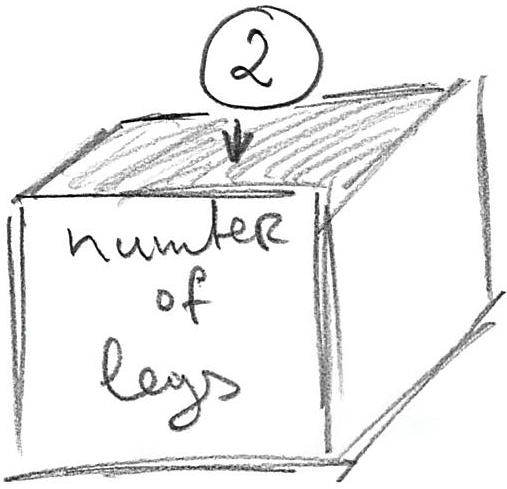
\includegraphics[width=0.5\linewidth]{images/variable-as-box} \end{center}

In Python würdest du schreiben

\begin{Shaded}
\begin{Highlighting}[]
\NormalTok{anzahl\_der\_beine }\OperatorTok{=} \DecValTok{2}
\end{Highlighting}
\end{Shaded}

Die obige \textbf{Zuweisungsanweisung} hat eine sehr einfache Struktur:

\begin{Shaded}
\begin{Highlighting}[]
\OperatorTok{\textless{}}\NormalTok{variablen}\OperatorTok{{-}}\NormalTok{name}\OperatorTok{\textgreater{}} \OperatorTok{=} \OperatorTok{\textless{}}\NormalTok{wert}\OperatorTok{\textgreater{}}
\end{Highlighting}
\end{Shaded}

Der Variablenname (das Namensschild auf der Kiste) sollte aussagekräftig sein, er kann mit Buchstaben oder \_ beginnen und kann Buchstaben, Zahlen und das Symbol \_ enthalten, aber keine Leerzeichen, Tabs, Sonderzeichen usw. Python empfiehlt\footnote{Naja, eigentlich \href{https://www.python.org/dev/peps/pep-0008/}{besteht} es darauf.} dass du die \textbf{snake\_case} Schreibweise (alles in Kleinbuchstaben, Unterstrich für Leerzeichen) verwendest, um deine Variablennamen zu formatieren. Der \texttt{\textless{}Wert\textgreater{}} auf der rechten Seite ist eine komplexere Geschichte, da er fest codiert sein kann (wie im obigen Beispiel), berechnet werden kann, indem andere Variablen oder dieselbe Variable, zurückgegeben von einer Funktion, usw. verwendet werden.

Die Verwendung von Variablen bedeutet, dass du dich auf die \textbf{Bedeutung} der entsprechenden Werte konzentrieren kannst, anstatt dir Sorgen darüber zu machen, was diese Werte sind. Beispielsweise kannst du das nächste Mal, wenn du etwas auf Grundlage der Anzahl der Beine eines Charakters berechnen musst (z.B., wie viele Paar Schuhe benötigt ein Charakter), dies auf Grundlage des aktuellen Wertes der Variablen \texttt{anzahl\_der\_beine} berechnen, anstatt anzunehmen, dass es \texttt{1} ist.

\begin{Shaded}
\begin{Highlighting}[]
\CommentTok{\# SCHLECHT: Warum 1? Ist es, weil der Character zwei Beine hat oder}
\CommentTok{\# weil wir jedem Character ein Paar Schuhe geben, unabhängig von}
\CommentTok{\# seiner tatsächlichen Anzahl von Beinen?}
\NormalTok{paar\_schuhe }\OperatorTok{=} \DecValTok{1}

\CommentTok{\# BESSER (aber was, wenn unser Charakter nur ein Bein hat?)}
\NormalTok{paar\_schuhe }\OperatorTok{=}\NormalTok{ anzahl\_der\_beine }\OperatorTok{/} \DecValTok{2}
\end{Highlighting}
\end{Shaded}

Variablen geben dir auch Flexibilität. Ihre Werte können sich während des Programmablaufs ändern: Der Punktestand des Spielers steigt, die Anzahl der Leben nimmt ab, die Anzahl der Zauber, die er wirken kann, steigt oder fällt je nach ihrem Einsatz, usw. Dennoch kannst du immer den Wert in der Variablen verwenden, um die notwendigen Berechnungen durchzuführen. Hier ist zum Beispiel ein leicht erweitertes Beispiel für \texttt{anzahl\_der\_schuhe}.

\begin{Shaded}
\begin{Highlighting}[]
\NormalTok{anzahl\_der\_beine }\OperatorTok{=} \DecValTok{2}

\CommentTok{\# ...}
\CommentTok{\# etwas passiert und unser Charakter wird in einen Tintenfisch verwandelt}
\NormalTok{anzahl\_der\_beine }\OperatorTok{=} \DecValTok{8}
\CommentTok{\# ...}

\CommentTok{\# der gleiche Code funktioniert immer noch und wir können immer noch die richtige Anzahl an Schuhpaaren berechnen}
\NormalTok{paar\_schuhe }\OperatorTok{=}\NormalTok{ anzahl\_der\_beine }\OperatorTok{/} \DecValTok{2}
\end{Highlighting}
\end{Shaded}

Wie bereits erwähnt, kannst du eine Variable als eine beschriftete Kiste betrachten, in die du etwas hineinlegen kannst. Das bedeutet, dass du immer den alten Wert ``wegwerfen'' und etwas Neues hineinlegen kannst. Im Falle von Variablen geschieht der ``Wegwerf''-Teil automatisch, da ein neuer Wert den alten überschreibt. Überprüfe selbst, welcher der endgültige Wert der Variable im unten stehenden Code ist?

\begin{Shaded}
\begin{Highlighting}[]
\NormalTok{anzahl\_der\_beine }\OperatorTok{=} \DecValTok{2}
\NormalTok{anzahl\_der\_beine }\OperatorTok{=} \DecValTok{5}
\NormalTok{anzahl\_der\_beine }\OperatorTok{=} \DecValTok{1}
\NormalTok{anzahl\_der\_beine}
\end{Highlighting}
\end{Shaded}

Mache Übung \#1.

Beachte, dass eine Variable (eine ``Kiste mit Namensschild'') erst existiert, nachdem du ihr etwas zugewiesen hast. Der folgende Code erzeugt also einen \texttt{NameError}, die Python-art zu sagen, dass sie noch nie von der Variable \texttt{anzahl\_der\_haende} gehört hat.

\begin{Shaded}
\begin{Highlighting}[]
\NormalTok{anzahl\_der\_beine }\OperatorTok{=} \DecValTok{2}
\NormalTok{anzahl\_der\_handschuhe }\OperatorTok{=}\NormalTok{ anzahl\_der\_haende }\OperatorTok{/} \DecValTok{2}
\end{Highlighting}
\end{Shaded}

Du kannst jedoch eine Variable erstellen, die keinen \emph{spezifischen} Wert hat, indem du ihr \texttt{None} zuweist. \texttt{None} wurde speziell für die Bedeutung \emph{kein Wert} oder \emph{nichts} zur Sprache hinzugefügt.

\begin{Shaded}
\begin{Highlighting}[]
\NormalTok{anzahl\_der\_haende }\OperatorTok{=} \VariableTok{None} \CommentTok{\# Die Variable existiert jetzt, hat aber keinen speziellen Wert.}
\end{Highlighting}
\end{Shaded}

Wie du bereits gesehen hast, kannst du einen Wert \emph{berechnen}, anstatt ihn anzugeben. Was wäre die Antwort hier?

\begin{Shaded}
\begin{Highlighting}[]
\NormalTok{anzahl\_der\_beine }\OperatorTok{=} \DecValTok{2} \OperatorTok{*} \DecValTok{2}
\NormalTok{anzahl\_der\_beine }\OperatorTok{=} \DecValTok{7} \OperatorTok{{-}} \DecValTok{2}
\NormalTok{anzahl\_der\_beine}
\end{Highlighting}
\end{Shaded}

Mache Übung \#2.

\hypertarget{zuweisungen-sind-keine-gleichungen}{%
\section{Zuweisungen sind keine Gleichungen!}\label{zuweisungen-sind-keine-gleichungen}}

\textbf{Sehr wichtig}: obwohl Zuweisungen \emph{wie} mathematische Gleichungen \emph{aussehen}, sind sie \textbf{keine Gleichungen!} Sie folgen einer \textbf{sehr wichtigen} Regel, die Sie im Kopf behalten müssen, wenn Sie Zuweisungen verstehen: die rechte Seite eines Ausdrucks wird \emph{zuerst} ausgewertet, bis der Endwert berechnet ist. Erst dann wird dieser Endwert der auf der linken Seite angegebenen Variable zugewiesen (also in die Kiste gelegt). Das bedeutet, dass Sie die gleiche Variable auf \emph{beiden} Seiten verwenden können! Sehen wir uns diesen Code an:

\begin{Shaded}
\begin{Highlighting}[]
\NormalTok{x }\OperatorTok{=} \DecValTok{2}
\NormalTok{y }\OperatorTok{=} \DecValTok{5}
\NormalTok{x }\OperatorTok{=}\NormalTok{ x }\OperatorTok{+}\NormalTok{ y }\OperatorTok{{-}} \DecValTok{4}
\end{Highlighting}
\end{Shaded}

Was passiert, wenn der Computer die letzte Zeile auswertet? Zunächst nimmt er die \emph{aktuellen} Werte aller Variablen (\texttt{2} für \texttt{x} und \texttt{5} für \texttt{y}) und setzt sie in den Ausdruck. Nach diesem internen Schritt sieht der Ausdruck so aus:

\begin{Shaded}
\begin{Highlighting}[]
\NormalTok{x }\OperatorTok{=} \DecValTok{2} \OperatorTok{+} \DecValTok{5} \OperatorTok{{-}} \DecValTok{4}
\end{Highlighting}
\end{Shaded}

Dann berechnet er den Ausdruck auf der rechten Seite und speichert, \textbf{sobald die Berechnung abgeschlossen ist}, diesen neuen Wert in \texttt{x}

\begin{Shaded}
\begin{Highlighting}[]
\NormalTok{x }\OperatorTok{=} \DecValTok{3}
\end{Highlighting}
\end{Shaded}

Machen Sie die Übung \#3, um sicherzugehen, dass Sie dies verstanden haben.

\hypertarget{constants}{%
\section{Konstanten}\label{constants}}

Obwohl die eigentliche Stärke von Variablen darin besteht, dass Sie ihren Wert ändern können, sollten Sie sie auch dann verwenden, wenn der Wert im gesamten Programm konstant bleibt. In Python gibt es keine echten Konstanten, sondern die Übereinkunft, dass ihre Namen vollständig \texttt{GROSSGESCHRIEBEN} sein sollten. Entsprechend wissen Sie, wenn Sie \texttt{SOLCH\_EINE\_VARIABLE} sehen, dass Sie ihren Wert nicht ändern sollten. Technisch gesehen ist das nur eine Empfehlung, denn niemand kann Sie davon abhalten, den Wert einer \texttt{KONSTANTE} zu ändern. Aber ein großer Teil der Benutzerfreundlichkeit von Python resultiert aus solchen Übereinkünften (wie der \texttt{snake\_case} Konvention oben). Wir werden später mehr von solchen Übereinkünften treffen, zum Beispiel beim Lernen über Objekte.

Unter Berücksichtigung all dessen, wenn die Anzahl der Beine im Spiel konstant bleibt, sollten Sie diese Konstanz betonen und schreiben

\begin{Shaded}
\begin{Highlighting}[]
\NormalTok{ANZAHL\_DER\_BEINE }\OperatorTok{=} \DecValTok{2}
\end{Highlighting}
\end{Shaded}

Ich empfehle dringend die Verwendung von Konstanten und vermeide das Hardcoding von Werten. Erstens, wenn Sie mehrere identische Werte haben, die verschiedene Dinge bedeuten (2 Beine, 2 Augen, 2 Ohren, 2 Fahrzeuge pro Figur, etc.), wird Ihnen eine \texttt{2} im Code nicht verraten, was diese \texttt{2} bedeutet (die Beine? Die Ohren? Der Punktemultiplikator?). Sie können das natürlich herausfinden, basierend auf dem Code, der diese Nummer verwendet, aber Sie könnten sich diese zusätzliche Mühe ersparen und stattdessen eine ordnungsgemäß benannte Konstante verwenden. Dann lesen Sie einfach ihren Namen und die Bedeutung des Wertes wird offensichtlich, und es ist die Bedeutung und nicht der tatsächliche Wert, der Sie hauptsächlich interessiert. Zweitens, wenn Sie entscheiden, diesen Wert dauerhaft zu \emph{ändern} (sagen wir, unsere Hauptfigur ist jetzt ein Dreifuß), bedeutet die Verwendung einer Konstante, dass Sie sich nur an einer Stelle Sorgen machen müssen, der Rest des Codes bleibt unverändert. Wenn Sie diese Zahl hart codiert haben, erwartet Sie eine aufregende \footnote{nicht wirklich} und definitiv lange Suche und Ersetzung im gesamten Code.

Machen Sie die Übung \#4.

\hypertarget{value-types}{%
\section{Datentypen}\label{value-types}}

Bisher haben wir nur ganzzahlige numerische Werte verwendet (1, 2, 5, 1000\ldots). Obwohl Python \href{https://docs.python.org/3/library/stdtypes.html}{viele verschiedene Datentypen} unterstützt, konzentrieren wir uns zunächst auf eine kleine Auswahl davon:

\begin{itemize}
\tightlist
\item
  Ganze Zahlen, die wir bereits verwendet haben, z.B. \texttt{-1}, \texttt{100000}, \texttt{42}.
\item
  Fließkommazahlen, die jeden realen Wert annehmen können, z.B. \texttt{42.0}, \texttt{3.14159265359}, \texttt{2.71828}.
\item
  Zeichenketten, die Text speichern können. Der Text ist zwischen entweder gepaarten Anführungszeichen \texttt{"einiger\ Text"} oder Apostrophen \texttt{\textquotesingle{}einiger\ Text\textquotesingle{}} eingeschlossen. Das bedeutet, dass Sie Anführungszeichen oder Apostrophe innerhalb der Zeichenkette verwenden können, solange sie von der Alternative umschlossen ist. Z.B., \texttt{"Schüleraufgaben"} (eingeschlossen in \texttt{"}, Apostroph \texttt{\textquotesingle{}} innen) oder \texttt{\textquotesingle{}"Alle\ Verallgemeinerungen\ sind\ falsch,\ auch\ diese."\ Mark\ Twain\textquotesingle{}} (Zitat von Apostrophen eingeschlossen). Es gibt noch viel mehr zu Zeichenketten und wir werden dieses Material im Laufe des Kurses behandeln.
\item
  Logische / boolesche Werte, die entweder \texttt{True} oder \texttt{False} sind.
\end{itemize}

Bei der Verwendung einer Variable ist es wichtig, dass Sie wissen, welchen Datentyp sie speichert, und das liegt meist bei Ihnen. In einigen Fällen wird Python einen Fehler ausgeben, wenn Sie versuchen, eine Rechnung mit inkompatiblen Datentypen durchzuführen. In anderen Fällen wird Python Werte automatisch zwischen bestimmten Typen konvertieren, z.B. ist jeder Ganzzahlwert auch ein Realwert, so dass die Konvertierung von \texttt{1} zu \texttt{1.0} meist trivial und automatisch ist. In anderen Fällen müssen Sie jedoch möglicherweise eine explizite Konvertierung verwenden. Gehen Sie zur Übung \#5 und versuchen Sie zu erraten, welcher Code laufen wird und welcher einen Fehler wegen inkompatiblen Typen werfen wird?

\begin{Shaded}
\begin{Highlighting}[]
\DecValTok{5} \OperatorTok{+} \FloatTok{2.0}
\CommentTok{\textquotesingle{}5\textquotesingle{}} \OperatorTok{+} \DecValTok{2}
\CommentTok{\textquotesingle{}5\textquotesingle{}} \OperatorTok{+} \StringTok{\textquotesingle{}2\textquotesingle{}}
\CommentTok{\textquotesingle{}5\textquotesingle{}} \OperatorTok{+} \VariableTok{True}
\DecValTok{5} \OperatorTok{+} \VariableTok{True}
\end{Highlighting}
\end{Shaded}

Mache Übung \#5.

Überrascht vom letzten? Das liegt daran, dass intern \texttt{True} auch \texttt{1} und \texttt{False} \texttt{0} ist!

Sie können explizit von einem Typ in einen anderen umwandeln, indem Sie spezielle Funktionen verwenden. Beispielsweise können Sie eine Zahl oder einen logischen Wert in einen String umwandeln, indem Sie einfach \href{https://docs.python.org/3/library/functions.html\#func-str}{str(\textless value\textgreater)} schreiben. Was wäre das Ergebnis in den untenstehenden Beispielen?

\begin{Shaded}
\begin{Highlighting}[]
\BuiltInTok{str}\NormalTok{(}\DecValTok{10} \OperatorTok{/} \DecValTok{2}\NormalTok{)}
\BuiltInTok{str}\NormalTok{(}\FloatTok{2.5} \OperatorTok{+} \VariableTok{True}\NormalTok{)}
\BuiltInTok{str}\NormalTok{(}\VariableTok{True}\NormalTok{)}
\end{Highlighting}
\end{Shaded}

Mache Übung \#6.

Ähnlich können Sie mit der Funktion \href{https://docs.python.org/3/library/functions.html\#bool}{bool(\textless value\textgreater)} in eine logische/boolesche Variable umwandeln. Die Regeln sind einfach, für numerische Werte ist \texttt{0} gleich \texttt{False}, jeder andere Nicht-Null-Wert wird in \texttt{True} umgewandelt. Für Zeichenketten wird eine leere Zeichenkette \texttt{\textquotesingle{}\textquotesingle{}} als \texttt{False} bewertet und eine nicht leere Zeichenkette wird in \texttt{True} umgewandelt. Was wäre die Ausgabe in den untenstehenden Beispielen?

\begin{Shaded}
\begin{Highlighting}[]
\BuiltInTok{bool}\NormalTok{(}\OperatorTok{{-}}\DecValTok{10}\NormalTok{)}
\BuiltInTok{bool}\NormalTok{(}\FloatTok{0.0}\NormalTok{)}

\NormalTok{secret\_message }\OperatorTok{=} \StringTok{\textquotesingle{}\textquotesingle{}}
\BuiltInTok{bool}\NormalTok{(secret\_message)}

\BuiltInTok{bool}\NormalTok{(}\StringTok{\textquotesingle{}False\textquotesingle{}}\NormalTok{)}
\end{Highlighting}
\end{Shaded}

Mache Übung \#7.

Die Umwandlung in Ganzzahlen oder Fließkommazahlen mit \href{https://docs.python.org/3/library/functions.html\#int}{int(\textless value\textgreater)} bzw. \href{https://docs.python.org/3/library/functions.html\#float}{float(\textless value\textgreater)} ist komplizierter. Der einfachste Fall ist von logisch auf Ganzzahl/Fließkommazahl, da \texttt{True} Ihnen \texttt{int(True)} ist \texttt{1} und \texttt{float(True)} ist \texttt{1.0} gibt und \texttt{False} gibt Ihnen \texttt{0}/\texttt{0.0}. Beim Umwandeln von Fließkommazahl auf Ganzzahl lässt Python einfach den Bruchteilteil fallen (es rundet nicht richtig!). Bei der Umwandlung einer Zeichenkette muss es sich um eine gültige Zahl des entsprechenden Typs handeln, sonst wird ein Fehler erzeugt. Sie können z. B. eine Zeichenkette wie \texttt{"123"} in eine Ganzzahl oder eine Fließkommazahl umwandeln, aber das funktioniert nicht für \texttt{"a123"}. Darüber hinaus können Sie \texttt{"123.4"} in eine Fließkommazahl umwandeln, aber nicht in eine Ganzzahl, da sie einen Bruchteil enthält. Angesichts all dessen, welche Zellen würden funktionieren und welche Ausgabe würden sie erzeugen?

\begin{Shaded}
\begin{Highlighting}[]
\BuiltInTok{float}\NormalTok{(}\VariableTok{False}\NormalTok{)}
\BuiltInTok{int}\NormalTok{(}\OperatorTok{{-}}\FloatTok{3.3}\NormalTok{)}
\BuiltInTok{float}\NormalTok{(}\StringTok{"67.8"}\NormalTok{)}
\BuiltInTok{int}\NormalTok{(}\StringTok{"123+3"}\NormalTok{)}
\end{Highlighting}
\end{Shaded}

Mache Übung \#8.

\hypertarget{print}{%
\section{Ausgabe drucken}\label{print}}

Um den Wert auszudrucken, müssen Sie die Funktion \href{https://docs.python.org/3/library/functions.html\#print}{print()} verwenden (wir werden später allgemein über Funktionen sprechen). Im einfachsten Fall übergeben Sie den Wert und er wird ausgegeben.

\begin{Shaded}
\begin{Highlighting}[]
\BuiltInTok{print}\NormalTok{(}\DecValTok{5}\NormalTok{)}
\CommentTok{\#\textgreater{} 5}
\end{Highlighting}
\end{Shaded}

oder

\begin{Shaded}
\begin{Highlighting}[]
\BuiltInTok{print}\NormalTok{(}\StringTok{"fünf"}\NormalTok{)}
\CommentTok{\#\textgreater{} fünf}
\end{Highlighting}
\end{Shaded}

Natürlich wissen Sie bereits über die Variablen Bescheid, also statt den Wert direkt einzugeben, können Sie stattdessen eine Variable übergeben und ihr \emph{Wert} wird ausgegeben.

\begin{Shaded}
\begin{Highlighting}[]
\NormalTok{anzahl\_der\_pfannkuchen }\OperatorTok{=} \DecValTok{10}
\BuiltInTok{print}\NormalTok{(anzahl\_der\_pfannkuchen)}
\CommentTok{\#\textgreater{} 10}
\end{Highlighting}
\end{Shaded}

oder

\begin{Shaded}
\begin{Highlighting}[]
\NormalTok{frühstück }\OperatorTok{=} \StringTok{"pfannkuchen"}
\BuiltInTok{print}\NormalTok{(frühstück)}
\CommentTok{\#\textgreater{} pfannkuchen}
\end{Highlighting}
\end{Shaded}

Sie können auch mehr als einen Wert/Variablen an die Druckfunktion übergeben und alle Werte werden nacheinander gedruckt. Wenn wir dem Benutzer zum Beispiel sagen wollen, was ich zum Frühstück hatte, können wir das tun

\begin{Shaded}
\begin{Highlighting}[]
\NormalTok{frühstück }\OperatorTok{=} \StringTok{"pfannkuchen"}
\NormalTok{anzahl\_der\_artikel }\OperatorTok{=} \DecValTok{10}
\BuiltInTok{print}\NormalTok{(frühstück, anzahl\_der\_artikel)}
\CommentTok{\#\textgreater{} pfannkuchen 10}
\end{Highlighting}
\end{Shaded}

Was wird von dem untenstehenden Code gedruckt?

\begin{Shaded}
\begin{Highlighting}[]
\NormalTok{abendessen }\OperatorTok{=} \StringTok{"steak"}
\NormalTok{zähler }\OperatorTok{=} \DecValTok{4}
\NormalTok{nachtisch }\OperatorTok{=} \StringTok{"muffins"}

\BuiltInTok{print}\NormalTok{(zähler, abendessen, zähler, nachtisch)}
\end{Highlighting}
\end{Shaded}

Mache Übung \#9.

Allerdings möchten Sie wahrscheinlich expliziter sein, wenn Sie die Informationen ausdrucken. Stellen Sie sich zum Beispiel vor, Sie haben diese drei Variablen:

\begin{Shaded}
\begin{Highlighting}[]
\NormalTok{mahlzeit }\OperatorTok{=} \StringTok{"Frühstück"}
\NormalTok{gericht }\OperatorTok{=} \StringTok{"Pfannkuchen"}
\NormalTok{anzahl }\OperatorTok{=} \DecValTok{10}
\end{Highlighting}
\end{Shaded}

Sie könnten natürlich \texttt{print(mahlzeit,\ gericht,\ anzahl)} machen, aber es wäre schöner, ``\emph{Ich hatte \textbf{10 Pfannkuchen} zum \textbf{Frühstück}}'' zu drucken, wobei die in Fettschrift gedruckten Elemente die eingefügten Variablenwerte wären. Dafür müssen wir die Formatierung von Zeichenketten verwenden. Bitte beachten Sie, dass die Formatierung von Zeichenketten nicht spezifisch für das Drucken ist, Sie können einen neuen Zeichenkettenwert über die Formatierung erstellen und ihn in einer Variable speichern, ohne ihn auszudrucken, oder ihn ausdrucken, ohne ihn zu speichern.

\hypertarget{string-formatting}{%
\section{Formatierung von Zeichenketten}\label{string-formatting}}

Eine großartige Ressource zur Formatierung von Zeichenketten in Python ist \href{https://pyformat.info/}{pyformat.info}. Da sich Python ständig weiterentwickelt, gibt es nun mehr als eine Art, Zeichenketten zu formatieren. Im Folgenden werde ich das ``alte'' Format vorstellen, das auf der klassischen Formatierung von Zeichenketten basiert, die in der Funktion \texttt{sprintf} in C, Matlab, R und vielen anderen Programmiersprachen verwendet wird. Es ist etwas weniger flexibel als neuere, aber für einfache Aufgaben ist der Unterschied vernachlässigbar. Das Wissen über das alte Format ist nützlich wegen seiner Allgemeinheit. Wenn Sie Alternativen lernen möchten, lesen Sie unter dem oben angegebenen Link.

Der allgemeine Aufruf lautet \texttt{"ein\ String\ mit\ Formatierung"\%(Tupel\ von\ Werten,\ die\ während\ der\ Formatierung\ verwendet\ werden)}. Sie werden später mehr über Tupel lernen. Gehen Sie im Moment davon aus, dass es sich einfach um eine durch Kommas getrennte Liste von Werten handelt, die in runden Klammern eingeschlossen sind: \texttt{(1,\ 2,\ 3)}.

In \texttt{"ein\ String\ mit\ Formatierung"}, geben Sie an, wo Sie den Wert mit dem Zeichen \texttt{\%} einfügen möchten, das von einer \emph{optionalen} Formatierungsinformation und dem \emph{erforderlichen} Symbol, das den \textbf{Typ} des Wertes definiert, gefolgt wird. Die Typsymbole sind

\begin{itemize}
\tightlist
\item
  \texttt{s} für Zeichenkette
\item
  \texttt{d} für eine Ganzzahl
\item
  \texttt{f} für einen Fließkommawert
\item
  \texttt{g} für einen ``optimal'' gedruckten Fließkommawert, so dass für große Werte die wissenschaftliche Notation verwendet wird (\emph{z.B.}, \texttt{10e5} statt \texttt{100000}).
\end{itemize}

Hier ist ein Beispiel, wie man einen String mit einer Ganzzahl formatiert:

\begin{Shaded}
\begin{Highlighting}[]
\BuiltInTok{print}\NormalTok{(}\StringTok{"Ich hatte }\SpecialCharTok{\%d}\StringTok{ Pfannkuchen zum Frühstück"}\OperatorTok{\%}\NormalTok{(}\DecValTok{10}\NormalTok{))}
\CommentTok{\#\textgreater{} Ich hatte 10 Pfannkuchen zum Frühstück}
\end{Highlighting}
\end{Shaded}

Sie sind nicht darauf beschränkt, einen einzigen Wert in einen String einzufügen. Sie können weitere Positionen über \texttt{\%} angeben, müssen jedoch sicherstellen, dass Sie die richtige Anzahl von Werten in der richtigen Reihenfolge übergeben. Können Sie vor dem Ausführen herausfinden, welcher Aufruf tatsächlich funktioniert (und was die Ausgabe sein wird) und welcher einen Fehler verursacht?

\begin{Shaded}
\begin{Highlighting}[]
\BuiltInTok{print}\NormalTok{(}\StringTok{\textquotesingle{}Ich hatte }\SpecialCharTok{\%d}\StringTok{ Pfannkuchen und entweder }\SpecialCharTok{\%d}\StringTok{ oder }\SpecialCharTok{\%d}\StringTok{ Steaks zum Abendessen\textquotesingle{}}\OperatorTok{\%}\NormalTok{(}\DecValTok{2}\NormalTok{))}
\BuiltInTok{print}\NormalTok{(}\StringTok{\textquotesingle{}Ich hatte }\SpecialCharTok{\%d}\StringTok{ Pfannkuchen und }\SpecialCharTok{\%d}\StringTok{ Steaks zum Abendessen\textquotesingle{}}\OperatorTok{\%}\NormalTok{(}\DecValTok{7}\NormalTok{, }\DecValTok{10}\NormalTok{))}
\BuiltInTok{print}\NormalTok{(}\StringTok{\textquotesingle{}Ich hatte }\SpecialCharTok{\%d}\StringTok{ Pfannkuchen und }\SpecialCharTok{\%d}\StringTok{ Steaks zum Abendessen\textquotesingle{}}\OperatorTok{\%}\NormalTok{(}\DecValTok{1}\NormalTok{, }\DecValTok{7}\NormalTok{, }\DecValTok{10}\NormalTok{))}
\end{Highlighting}
\end{Shaded}

Machen Sie Übung \#10.

Wie oben erwähnt, haben Sie im Falle von echten Werten zwei Möglichkeiten: \texttt{\%f} und \texttt{\%g}. Letzterer verwendet die wissenschaftliche Notation (z.B. \texttt{1e10} für \texttt{10000000000}), um eine Darstellung kompakter zu machen.

Machen Sie Übung \#11, um ein besseres Gefühl für den Unterschied zu bekommen.

Es gibt noch viel mehr zur Formatierung und Sie können auf \href{https://pyformat.info/}{pyformat.info} darüber lesen. Diese Grundlagen sind jedoch ausreichend, um in dem nächsten Kapitel mit der Programmierung unseres ersten Spiels zu beginnen.

  \bibliography{book.bib}

\end{document}
